\documentclass[10pt]{beamer}

\usepackage[utf8]{inputenc}
\usepackage{enumitem, environ, marvosym, pgfplots, siunitx, xspace}
\usetikzlibrary{arrows.meta,   	        	% big arrows
				calc,						% coordinates calculations
				decorations.markings,		% in-line arrows
				overlay-beamer-styles,		% for vsible on=<> overlays
				positioning,				% place nodes
				}
\usepgfplotslibrary{groupplots}

%% Lengths

% base unit for coordinates
\newlength\quantum
\newlength\quanta
\setlength\quantum{3pt}
\setlength\quanta{\quantum}

% slides dimensions = N * quantum,
% ratio 120/90 = 4/3, with 3 quanta
% for the footline
\setlength{\paperwidth}{120\quanta}
\setlength{\paperheight}{93\quanta}

% set a footline with total height (height + depth) of 3 quanta
\newlength\tinyxheight
\newlength\flheight
\newlength\fldepth
\settoheight{\tinyxheight}{\tiny x}
\setlength\flheight{\dimexpr 1.5\quantum + 0.5\tinyxheight \relax}
\setlength\fldepth{\dimexpr 1.5\quantum - 0.5\tinyxheight \relax}

% width of a column in a five (V) columns layout
\newlength\colv
\newlength\colvsep  % including the inter-column spacing
\setlength\colv{17.6\quanta}
\setlength\colvsep{\dimexpr\colv + \baselineskip\relax}

% big column width (two columns + one baseline skip)
\newlength\bigcol
\newlength\halfbigcol
\setlength\bigcol{\dimexpr 2\colv + \baselineskip\relax}
\setlength\halfbigcol{0.5\bigcol}

% depth in Large fonts, for positioning titles
\newlength\Largeydepth
\settodepth{\Largeydepth}{\Large y}

% M height in footnotesize fonts, for positioning tick labels
\newlength\ssMheight
\settoheight{\ssMheight}{\scriptsize M}

% temporary lengths to locally replace long length calculations
\newlength\templen
\newlength\buffer

% map layout
\newlength\w
\newlength\e

%% lists stuff
\newenvironment{listed}{
	\begin{itemize}[nosep]
	\setlength\itemsep{2\quanta}  % adds to the existing baseline skip
	}{
	\end{itemize}
	}

% remove indentation
\settowidth{\leftmargini}{\usebeamertemplate{itemize item}}
\addtolength{\leftmargini}{.36\labelsep} % narrower than usual item symbol

%% Overall style

\colorlet{col}{orange}  % main color
% map colors
\colorlet{hls1}{black}
\colorlet{hls2}{black}
\colorlet{hls3}{black}

% square bullet items
\setbeamertemplate{itemize item}[square]
\setbeamercolor{itemize item}{fg=col}

% enumitem overrides beamer settings,
% so list styles have to be re-specified
\setitemize{label=\usebeamerfont*{itemize item}%
  \usebeamercolor[fg]{itemize item}
  \usebeamertemplate{itemize item}}



%% TikZ based slide template

% slide environment composed of a TikZ picture
% with the following nodes
%
% (NW) ----- (N) ----- (NE)
%   |         |         |
%   |         |         |
%  (W) ----- (C) ----- (E)
%   |         |         |
%   |         |         |
% (SW) ----- (S) ----- (SE)

\NewEnviron{slide}[1][]{%
\begin{frame}[t]%
	\makebox[\textwidth][c]{%
		\begin{tikzpicture}[overlay, remember picture, inner sep=0pt]%
		
		\node (N) at (page cs:0,45) {};
		\node (S) at (page cs:0,-45) {};
		\node (W) at (page cs:-60,0) {};
		\node (E) at (page cs:60,0) {};
		\node (NW) at (page cs:-60,45) {};
		\node (NE) at (page cs:60,45) {};
		\node (SW) at (page cs:-60,-45) {};
		\node (SE) at (page cs:60,-45) {};
		\node (C) at (page cs:0,0) {};
		
		\node[anchor=north west, align=left, font=\Large, black!80,
			  yshift=\Largeydepth+.95pt, xshift=-.95pt] (title)
			at (page cs:-52,37) {#1};
			
			\normalsize\BODY
		
		\end{tikzpicture}}%
\end{frame}}

% draw help lines
\newcommand\drawhelplines{
	% title top lines
	\draw[teal] (page cs:-60,37) -- (page cs:60,37)
				(page cs:-60,31) -- (page cs:60,31);
	% pictures grid
	\draw[gray] foreach \c in {0,...,4}{
				(p5cl cs:\c,0)  -- (p5cl cs:\c,15)
				(p5cr cs:\c,0)  -- (p5cr cs:\c,15)
					foreach \l in {0,...,15}{
						(p5cl cs:\c,\l)  -- (p5cr cs:\c,\l)}};
	% text grid
	\draw[teal] foreach \c in {0,...,4}{
					foreach \l in {0,...,14}{
						(t5cl cs:\c,\l)  -- (t5cr cs:\c,\l)}};
	% margin
	\draw[col] (p5cr cs:1,-2) node (x) {} -- (x |- N);}

% draw full grid
\newcommand\drawfullgrid{
	\draw[gray] foreach \x in {-60,...,60}{
					(page cs:\x,-45) -- (page cs:\x,45)}
				foreach \y in {-45,...,45}{
					(page cs:-60,\y) -- (page cs:60,\y)};}



% Environment for map and title page
\NewEnviron{maplayout}{

\begin{frame}[plain, noframenumbering]
\makebox[\textwidth][c]{
\begin{tikzpicture}[overlay, remember picture, inner sep=0pt]%

% main title
\node [anchor=base west, align=left, font=\LARGE, black!80]
	at (page cs:-44,23) {Modélisation de pompes à chaleur\\
						 air-air à capacité variable (PàCCV)};

% test bench icon
\filldraw [hls1!30] (p5cl cs:0,10)++(8\quanta,0) -| ++(7\quanta,5\quanta)
	-- ++(-3.5\quanta,3\quanta) -- ++(-3.5\quanta,-3\quanta) -- cycle;
\filldraw [hls1!30] (p5cr cs:0,10)++(8\quanta,0) -- ++(0,5\quanta) --
	++(-3.5\quanta,3\quanta) -- ++(-3.5\quanta,-3\quanta) |- cycle;
\draw [very thick, hls1!30]
	(p5cl cs:0,10)++(15\quanta,\quantum) coordinate (C1)
	-- +(\colv-14\quanta,0)
	(C1)++(0,2\quanta) -- +(\colv-14\quanta,0);


% control icon
\setlength\templen{0.8\baselineskip}

\begin{scope}[shift={($(p5cl cs:0,6)+(8\quanta,0)$)},
			  x=2\baselineskip, y=2\baselineskip]

\setlength\w{1.2\templen}
\setlength\e{\dimexpr \colv - 4\w \relax}

\draw [hls2!30, -{Stealth[scale=.5]}, thick]
	(0,0.8) -- ++(\w,0) ++(\w,0) -- ++(\e,0) ++(\w,0) -- ++(\w,0);
\filldraw [hls2!30] (\w,1) rectangle ++(\w,-\templen)
				 (2\w+\e,1) rectangle ++(\w,-\templen)
				 (.5\colv+.4\w,0) -- coordinate (Ain) ++(0,\templen) --
				 ++(-.8\w,-.5\templen) -- cycle;
\draw [hls2!30, -{Stealth[scale=.5]}, thick]
	(\colv-.5\w,.8) |- (Ain) ++(-.8\w,0) -| (.5\w,.8);


\end{scope}


% performance icon
\begin{scope}[shift={($(p5cl cs:0,2)+(8\quanta,0)$)},
			  x=2\baselineskip, y=2\baselineskip]

\setlength\buffer{0.48\baselineskip}
\filldraw [hls3!30]
	foreach \X in {0,1}{
	 	foreach \Y in {0,1}{
	 		foreach \x in {0,1}{
	 			foreach \y in {0,1}{
		(\X*1.2*\baselineskip, \Y*1.2*\baselineskip)++(\x\buffer,\y\buffer)
		rectangle ++(0.4\templen,0.4\templen)}}}};

\draw [hls3!30, thick] (\colv,0)++(-1,0) coordinate (O) -- ++(1,1);
\draw [semithick, hls3!30] (\colv,0) -| ++(-1,1);
\foreach \Point in {{.2,.15}, {.2,.3}, {.3,.31}, {.4,.34}, {.4,.55},
					{.55,.47}, {.6,.75}, {.7,.45}, {.75,.6}, {.8,.9},
					{.9,.97}}{
	\node [dot, scale=.7, hls3!30] at ($(O)+(\Point)$) {};}

\end{scope}


\BODY


\fill (page cs:-60,-45) rectangle (page cs:60,-48);

\end{tikzpicture}}
\end{frame}
}



% map[i] highlights section i
\newcommand{\map}[1][0]{

\pgfmathparse{
    ifthenelse(#1==1, "col", "black")}%
\colorlet{hls1}{\pgfmathresult}
\pgfmathparse{
    ifthenelse(#1==2, "col", "black")}%
\colorlet{hls2}{\pgfmathresult}
\pgfmathparse{
    ifthenelse(#1==3, "col", "black")}%
\colorlet{hls3}{\pgfmathresult}

\begin{maplayout}

\node[anchor=base east, hls1!60] at (t5cr cs:1,11) {1};
\node[anchor=base west, hls1] at (t5cl cs:2,11)
	{Collecter les données adéquates};
\node[anchor=base west, hls1!60] at (t5cl cs:2,10)
	{\footnotesize Banc d'essai et calcul des capacités};

\node[anchor=base east, hls2!60] at (t5cr cs:1,7) {2};
\node[anchor=base west, hls2] at (t5cl cs:2,7) {Modéliser le contrôle};
\node[anchor=base west, hls2!60] at (t5cl cs:2,6)
	{\footnotesize Fréquence, mode d'opération et dégivrage};

\node[anchor=base east, hls3!60] at (t5cr cs:1,3) {3};
\node[anchor=base west, hls3] at (t5cl cs:2,3)
	{Compléter les performances};
\node[anchor=base west, hls3!60] at (t5cl cs:2,2)
	{\footnotesize Corrections pour la fréquence et l'humidité};

\end{maplayout}
}




%% Plot options
\pgfkeys{/pgfplots/plot options/.style={
    separate axis lines,
    enlargelimits=false,
    axis x line*=bottom,
    axis x line shift=4\quanta,
    axis y line shift=4\quanta,
    axis y line*=left,
    scale only axis,
    ticklabel style={color=gray},
    tickwidth=\quantum,
    axis line style={gray!80!white, semithick},
    major tick style={gray!80!white, semithick},
    ticklabel style={font=\scriptsize},
    xticklabel style={yshift=\ssMheight-3\quanta},
    yticklabel style={xshift=\ssMheight-3\quanta},}}



%% Footline

% white on black footline, to set it apart from the slide
\setbeamercolor{head/foot}{fg=white, bg=black}
\setbeamertemplate{footline}{
\begin{beamercolorbox}[wd=\paperwidth,
					   ht=\flheight,
					   dp=\fldepth]{head/foot}
%	\makebox[.3333\paperwidth]{\insertsection}
%	\makebox[.3333\paperwidth]{\itshape\insertsubsection}
	\hspace*{8\quanta}\insertsection{}
	\hfill\insertframenumber{}\hspace*{8\quanta}
\end{beamercolorbox}%
}
\beamertemplatenavigationsymbolsempty  % remove navigation symbols


%% Quantities
\newcommand{\xmath}[1]{\ensuremath{#1}\xspace}  % ensure math mode

\newcommand{\Qh}[1][]{\xmath{\skew{5}\dot Q_{\text{h}#1}}}
\newcommand{\Qc}{\xmath{\skew{5}\dot Q_\text{c}}}
\newcommand{\Qcs}{\xmath{\skew{5}\dot Q_\text{cs}}}
\newcommand{\Qcl}{\xmath{\skew{5}\dot Q_\text{cl}}}
\newcommand{\Qca}{\xmath{\skew{5}\dot Q}}
\newcommand{\Pel}{\xmath{P_\text{el}}}
\newcommand{\Pcp}{\xmath{P_\text{comp}}}
\newcommand{\Pfi}{\xmath{P_\text{fi}}}
\newcommand{\fc}[1][]{\xmath{f_{c#1}}}
\newcommand{\fcn}[1][]{\xmath{\nu_{#1}}}
\newcommand{\Tr}[1][]{\xmath{T_{r#1}}}
\newcommand{\Twbr}[1][]{\xmath{T_{{\text{wb}r#1}}}}
\newcommand{\Ts}{\xmath{T_s}}
\newcommand{\To}[1][]{\xmath{T_{o#1}}}
\newcommand{\Tset}{\xmath{T_\text{set}}}
\newcommand{\dTr}{\xmath{\Delta T_r}}
\newcommand{\mr}{\xmath{\skew{5}\dot m_\text{r}}}
\newcommand{\ma}[1][]{\xmath{\skew{5}\dot m_{\text{a}#1}}}
\newcommand{\tdf}{\xmath{\tau_\text{df}}}
\newcommand{\trec}{\xmath{\tau_\text{rec}}}
\newcommand{\tss}{\xmath{\tau_\text{ss}}}
\newcommand{\theat}{\xmath{\tau_\text{h}}}
\newcommand{\Va}[1][]{\xmath{\skew{3}\dot V_{\hskip-1pt\text{a}#1}}}
\newcommand{\nph}[1]{\xmath{\varphi_\text{h#1}}}
\newcommand{\npc}[1]{\xmath{\varphi_\text{c#1}}}
\newcommand{\npcs}[1]{\xmath{\varphi_\text{cs#1}}}
\newcommand{\npcl}[1]{\xmath{\varphi_\text{cl#1}}}

% Define a new coordinate system for the page:
%
% (-60,45)-----(0,45)------(6,45)
%	  |			 |			 |
%	  |			 |			 |
% (-60,0)------(0,0)------(60,0)
%	  |			 |			 |
%	  |			 |			 |
% (-60,-45)----(0,-45)----(60,-45)
%
\makeatletter
\def\parsecomma#1,#2\endparsecomma{\def\page@x{#1}\def\page@y{#2}}
\tikzdeclarecoordinatesystem{page}{
    \parsecomma#1\endparsecomma
    \pgfpointanchor{current page}{north east}
    % Save the upper right corner
    \pgf@xc=\pgf@x%
    \pgf@yc=\pgf@y%
    % save the lower left corner (excluding footline)
    \pgfpointanchor{current page}{south west}
    \pgf@xb=\pgf@x%
    \pgf@yb=\dimexpr\pgf@y+3\quanta\relax%
    % Transform to the correct placement
    \pgfmathparse{(\pgf@xc-\pgf@xb)/120.*\page@x+(\pgf@xc+\pgf@xb)/2.}
    \expandafter\pgf@x\expandafter=\pgfmathresult pt
    \pgfmathparse{(\pgf@yc-\pgf@yb)/90.*\page@y+(\pgf@yc+\pgf@yb)/2.}
    \expandafter\pgf@y\expandafter=\pgfmathresult pt}
\makeatother


% Five column layouts (pictures/text and left/right)
%    l:(0,N)	  r:(0,N) l:(1,N)   r:(1,N) l:(2,N)   r:(2,N)
%	  +-----------+		+-----------+	  +-----------+
%	  |			  |		|			|	  |			  |
%	  +-----------+		+-----------+	  +-----------+
%	  |			  |		|			|	  |			  |
%	  +-- col 0 --+		+-- col 1 --+	  +-- col 2 --+   ...
%	  |			  |		|			|	  |			  |
%	  +-----------+		+-----------+	  +-----------+
%	  |			  |		|			|	  |			  |
%	  +-----------+		+-----------+	  +-----------+
%    l:(0,0)	  r:(0,0) l:(1,0)   r:(1,0) l:(2,0)   r:(2,0)
\makeatletter
\def\parsecomma#1,#2\endparsecomma{\def\page@x{#1}\def\page@y{#2}}
\tikzdeclarecoordinatesystem{p5cl}{
    \parsecomma#1\endparsecomma
    \pgfpointanchor{current page}{south west}
    % Save the upper right corner
    \pgf@xc=\dimexpr\pgf@x+3\baselineskip+\colv\relax%
    \pgf@yc=\dimexpr\pgf@y+11\quanta+15\baselineskip\relax%
    % save the lower left corner
    \pgf@xb=\dimexpr\pgf@x+2\baselineskip\relax%
    \pgf@yb=\dimexpr\pgf@y+11\quanta\relax%
    % Transform to the correct placement
    \pgfmathparse{(\pgf@xc-\pgf@xb)*\page@x+\pgf@xb}
    \expandafter\pgf@x\expandafter=\pgfmathresult pt
    \pgfmathparse{(\pgf@yc-\pgf@yb)/15.*\page@y+\pgf@yb}
    \expandafter\pgf@y\expandafter=\pgfmathresult pt}
\tikzdeclarecoordinatesystem{p5cr}{
    \parsecomma#1\endparsecomma
    \pgfpointanchor{current page}{south west}
    % Save the upper right corner
    \pgf@xc=\dimexpr\pgf@x+3\baselineskip+2\colv\relax%
    \pgf@yc=\dimexpr\pgf@y+11\quanta+15\baselineskip\relax%
    % save the lower left corner
    \pgf@xb=\dimexpr\pgf@x+2\baselineskip+\colv\relax%
    \pgf@yb=\dimexpr\pgf@y+11\quanta\relax%
    % Transform to the correct placement
    \pgfmathparse{(\pgf@xc-\pgf@xb)*\page@x+\pgf@xb}
    \expandafter\pgf@x\expandafter=\pgfmathresult pt
    \pgfmathparse{(\pgf@yc-\pgf@yb)/15.*\page@y+\pgf@yb}
    \expandafter\pgf@y\expandafter=\pgfmathresult pt}
\tikzdeclarecoordinatesystem{t5cl}{
    \parsecomma#1\endparsecomma
    \pgfpointanchor{current page}{south west}
    % Save the upper right corner
    \pgf@xc=\dimexpr\pgf@x+3\baselineskip+\colv\relax%
    \pgf@yc=\dimexpr\pgf@y+12\quanta+15\baselineskip\relax%
    % save the lower left corner
    \pgf@xb=\dimexpr\pgf@x+2\baselineskip\relax%
    \pgf@yb=\dimexpr\pgf@y+12\quanta\relax%
    % Transform to the correct placement
    \pgfmathparse{(\pgf@xc-\pgf@xb)*\page@x+\pgf@xb}
    \expandafter\pgf@x\expandafter=\pgfmathresult pt
    \pgfmathparse{(\pgf@yc-\pgf@yb)/15.*\page@y+\pgf@yb}
    \expandafter\pgf@y\expandafter=\pgfmathresult pt}
\tikzdeclarecoordinatesystem{t5cr}{
    \parsecomma#1\endparsecomma
    \pgfpointanchor{current page}{south west}
    % Save the upper right corner
    \pgf@xc=\dimexpr\pgf@x+3\baselineskip+2\colv\relax%
    \pgf@yc=\dimexpr\pgf@y+12\quanta+15\baselineskip\relax%
    % save the lower left corner
    \pgf@xb=\dimexpr\pgf@x+2\baselineskip+\colv\relax%
    \pgf@yb=\dimexpr\pgf@y+12\quanta\relax%
    % Transform to the correct placement
    \pgfmathparse{(\pgf@xc-\pgf@xb)*\page@x+\pgf@xb}
    \expandafter\pgf@x\expandafter=\pgfmathresult pt
    \pgfmathparse{(\pgf@yc-\pgf@yb)/15.*\page@y+\pgf@yb}
    \expandafter\pgf@y\expandafter=\pgfmathresult pt}
\makeatother
\makeatletter

\pgfdeclareshape{triangle}{
	\inheritsavedanchors[from=rectangle]
	\inheritanchorborder[from=rectangle]
	\inheritanchor[from=rectangle]{north}
	\inheritanchor[from=rectangle]{north west}
	\inheritanchor[from=rectangle]{north east}
	\inheritanchor[from=rectangle]{center}
	\inheritanchor[from=rectangle]{west}
	\inheritanchor[from=rectangle]{east}
	\inheritanchor[from=rectangle]{mid}
	\inheritanchor[from=rectangle]{mid west}
	\inheritanchor[from=rectangle]{mid east}
	\inheritanchor[from=rectangle]{base}
	\inheritanchor[from=rectangle]{base west}
	\inheritanchor[from=rectangle]{base east}
	\inheritanchor[from=rectangle]{south}
	\inheritanchor[from=rectangle]{south west}
	\inheritanchor[from=rectangle]{south east}
	\backgroundpath{
		% store lower right in xa/ya and upper right in xb/yb
		\southwest \pgf@xa=\pgf@x \pgf@ya=\pgf@y
		\northeast \pgf@xb=\pgf@x \pgf@yb=\pgf@y
		% construct main path
		\pgfpathmoveto{\pgfpoint{\pgf@xa}{\pgf@ya}}
		\pgfpathlineto{\pgfpoint{0.5\pgf@xb+0.5\pgf@xa}{\pgf@yb}}
		\pgfpathlineto{\pgfpoint{\pgf@xb}{\pgf@ya}}
		\pgfpathclose}}

\makeatother

\tikzstyle{becomes} = [triangle, col!50, minimum width=4\quanta,
					   minimum height=2\quanta, fill]
\tikzstyle{dot} = [circle, fill, scale=.3, inner sep=3pt]
\tikzstyle{sum} = [circle, fill=gray!50, inner sep=3pt]
\tikzstyle{block} = [rectangle, fill=gray!50, inner sep=5pt]

\tikzset{
	fan/.pic={
		\path[draw, join=round] (0,0) arc (140:40:#1/2) arc (320:220:#1/2)
						  arc (40:140:#1/2) arc (220:320:#1/2);},
	fan2/.pic={
		\path[draw, join=round] (0,0) arc (110:70:#1/2) arc (290:250:#1/2)
						  arc (70:110:#1/2) arc (250:290:#1/2);}}


\tikzset{
	midarrow/.style args={#1-#2}{
		postaction=decorate,
		decoration={
			markings,
			mark=at position #1 with {\arrow{#2}}}}}

\tikzstyle{HX} = [decorate, decoration = {zigzag,
										  segment length = 2.5mm,
										  amplitude = 1mm}]

\tikzstyle{expValve} = [hourglass, draw,
						minimum height=4mm, minimum width=2mm]

\tikzset{
	hl/.style args={#1 on #2}{
		background default #1=black,
		background #1=col,
		#1 on=#2},
	hlg/.style args={#1 on #2}{
		background default #1=gray!50,
		background #1=col,
		#1 on=#2},
	hlb/.style args={#1 on #2}{
		background default #1=gray,
		background #1=black,
		#1 on=#2},
	hlbg/.style args={#1 on #2}{
		background default #1=gray!50,
		background #1=col!50,
		#1 on=#2}}



\begin{document}


\begin{frame}[plain, noframenumbering]
\makebox[\textwidth][c]{
\begin{tikzpicture}[overlay, remember picture, inner sep=0pt]%


\node[anchor=base west, align=left, font=\LARGE] at (page cs:-44,23)
	{Modélisation de pompes à chaleur\\air-air à capacité variable (PàCCV)};

\node[anchor=north east] at (page cs:44,11)
	{\includegraphics[width=\dimexpr0.5\colv+\colvsep\relax]{pictures/logo-poly.pdf}};

\node[anchor=base east] at (page cs:44, -8) {Gregor Strugala};
\node[anchor=base east] at (page cs:44, -24) {\color{gray} 22 mai 2019};

\fill (page cs:-60,-45) rectangle (page cs:60,-48);

\end{tikzpicture}}
\end{frame}


\begin{frame}[plain, noframenumbering]
\makebox[\textwidth][c]{
\begin{tikzpicture}[overlay, remember picture, inner sep=0pt]%


\node[anchor=base west, align=left, font=\LARGE] at (page cs:-44,23)
	{Modélisation de pompes à chaleur\\air-air à capacité variable (PàCCV)};

\node[anchor=base west] at (t5cr cs:2,11) {1};
\node[anchor=base west] at (t5cl cs:3,11) {Banc d'essai};
\node[anchor=base west, gray] at (t5cl cs:3,10) {\footnotesize Sous-titre};

\node[anchor=base west] at (t5cr cs:2,7) {2};
\node[anchor=base west] at (t5cl cs:3,7) {Contrôle};
\node[anchor=base west, gray] at (t5cl cs:3,6) {\footnotesize Sous-titre};

\node[anchor=base west] at (t5cr cs:2,3) {3};
\node[anchor=base west] at (t5cl cs:3,3) {Performance};
\node[anchor=base west, gray] at (t5cl cs:3,2) {\footnotesize Sous-titre};

\fill (page cs:-60,-45) rectangle (page cs:60,-48);

\end{tikzpicture}}
\end{frame}


% Illustration and advantages of variable capacity
\begin{slide}[Les PàCCV adaptent leur capacité aux besoins\\
			  pour fonctionner de façon continue]

% Illustration
\only<1>{
\node[anchor=mid west, align=left] at (p5cl cs:1,11) {capacité\\fixe};
\node[anchor=mid west, align=left] at (p5cl cs:1,3) {capacité\\variable};

\begin{scope}[shift={(p5cr cs:1,10)},
			  x=\bigcol/6+\baselineskip/6, y=3\baselineskip]

\draw[semithick] (0,.3333333) -- (3,.33333333) |- (6,.666666);
\draw[col, very thick]
	  (0,0) .. controls (0.1, 1) and (0.2, 1) .. (0.5,1)
   -- (0.5,1) .. controls (0.52, 0) and (0.6, 0) .. (0.7,0)
   -- (1.5,0) .. controls (1.6, 1) and (1.7, 1) .. (2,1)
   -- (2,1) .. controls (2.02, 0) and (2.1, 0) .. (2.2,0)
   -- (3,0) .. controls (3.1, 1) and (3.2, 1) .. (3.5,1)
   -- (4,1) .. controls (4.02, 0) and (4.1, 0) .. (4.2,0)
   -- (4.5,0) .. controls (4.6, 1) and (4.7, 1) .. (5,1)
   -- (5.5,1) .. controls (5.52, 0) and (5.6, 0) .. (5.7,0) -- (6,0);
	
\end{scope}


\node[becomes, rotate=180] at (p5cr cs:2,7.5) {};


\begin{scope}[shift={(p5cr cs:1,2)},
			  x=\bigcol/6+\baselineskip/6, y=\baselineskip]

\draw[semithick] (0,1) -- (3,1) |- (6,2);
\def\phase{46.87329}  % found numerically with scipy
\draw[col, very thick] plot[domain=0:3, samples=100, smooth]
			(\x, {1 - exp(-2*\x) * cos(700*\x + \phase) / cos(\phase)});
	
\end{scope}


\begin{scope}[shift={($(p5cr cs:1,3)+(\colv+\baselineskip,0)$)},
			  x=\bigcol/6+\baselineskip/6, y=\baselineskip]

% use rect line cap for joining but clip the part sticking out
\clip (p5cr cs:1,3) rectangle ++(2\colvsep,3\baselineskip);
\def\phase{46.87329}
\draw[col, very thick, line cap=rect] plot[domain=0:3, samples=100, smooth]
			(\x, {1 - exp(-2*\x) * cos(700*\x + \phase) / cos(\phase)});
\end{scope}
}


% Advantages
\only<2->{
\node[anchor=base west, align=left] (list) at (t5cr cs:1,5){
	\begin{minipage}[b]{2\colvsep}
	\hskip-.8pt Et ainsi elles augmentent\\
	\begin{listed}
        \item la performance
        \item la plage de températures
    \end{listed}
    \end{minipage}};
}

\end{slide}



% Étude de cas
\begin{slide}[Un modèle dynamique adéquat est nécessaire\\
			  pour simuler correctement les PàCCV]

\node[anchor=base west] (text) at (t5cl cs:0,4) {
	\begin{minipage}[b]{\dimexpr2\colvsep+4\quanta}\raggedright
		\emph{Exemple}\\[2\baselineskip]
		Profil de consommation\\d'une unité de résidence typique,\\~\\
		avec un pas de temp $ \Delta t = \SI{1}{\minute} $
	\end{minipage}};

\node[anchor=south east] at (p5cr cs:4,3)
	{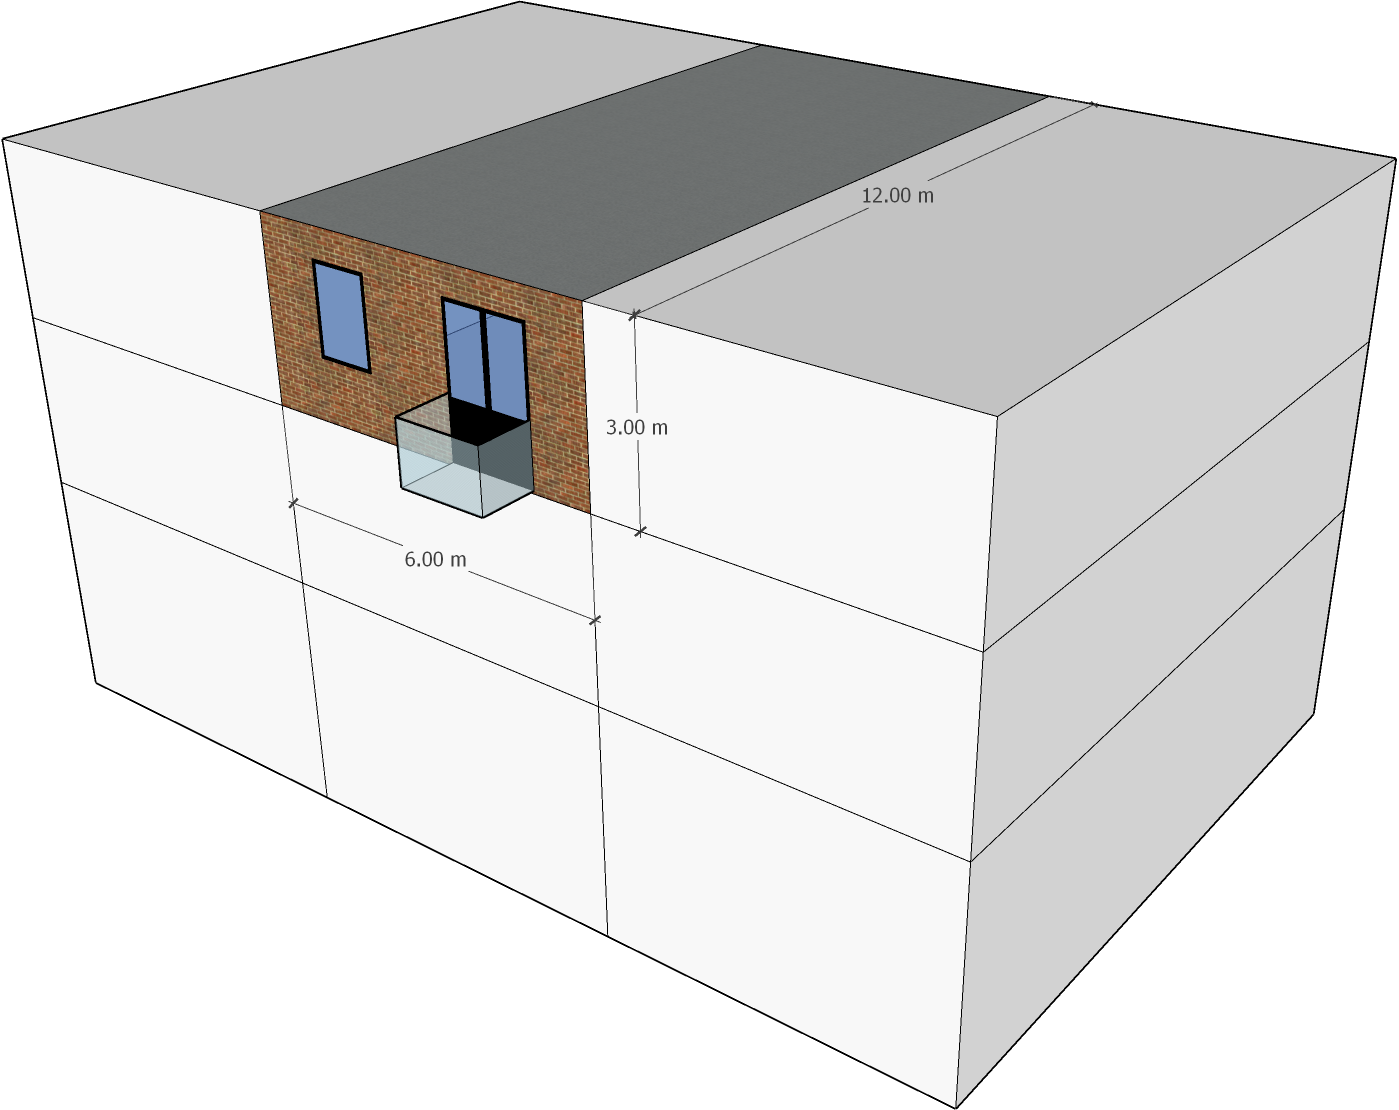
\includegraphics[height=9\baselineskip]{pictures/plex-unit}};

\end{slide}



% Données incomplètes
\begin{slide}[Les manufacturiers ne donnent pas suffisamment\\
			  d'informations sur les performances%
			  \only<5->{, ni sur le contrôle}]

\only<1>{
\begin{axis}[plot options, clip=false,
			 at={(p5cl cs:2,2)},
			 width=\bigcol+2\baselineskip, height=12\baselineskip,
			 xtick={-26.1, 15},
			 xticklabels={\num{-26.1}\phantom{$-$},
			 			  \phantom{\,\si{\celsius}}\SI{15}{\celsius}},
			 ytick={1.42, 4.75},]
\foreach \i in {1, ..., 4}{
	\addplot[mark=*, mark size=1pt, semithick] table[x=Toa, y=COP_at_T\i]
		{data/manu-data-heating.tsv};}
\foreach \i/\COP in {1/4.75, 2/4.524, 3/4.339, 4/3.961}{%
	\edef\temp{\noexpand\node (T\i) at (axis cs:15,\COP) {};}
	\temp}
\end{axis}
\node[anchor=mid west, font=\footnotesize] at (p5cl cs:1,14) {COP};
\node[anchor=base east, font=\footnotesize] (Toa)
	at (t5cr cs:4,0) {\To};
\foreach \i/\Ti in {1/15.6, 2/18.3, 3/21.1, 4/23.8}{
	\node[font=\footnotesize, gray, anchor=east] (Tr\i)
		at (T\i -| Toa.east) {\SI{\Ti}{\celsius}};
	\draw[gray] (T\i)++(4.5pt,0) -- ($(Tr\i.west)-(4pt,0)$);}
\node[anchor=west, yshift=-2\baselineskip, font=\footnotesize]
	at (Tr4.west) {\Tr};
}

\def\displayat{2}
\foreach \row/\rowlabel in {0/3, 1/2, 2/1}{
	\foreach \col/\collabel in {2/1, 3/2, 4/3}{
		\colorlet{background}{gray!10}
		\ifnum \row=2
			\ifnum \col=2
				\temporal<3>{
					\colorlet{background}{gray!10}}{
					\colorlet{background}{gray!10}}{
					\colorlet{background}{col!20}}
			\fi
		\fi
		\ifnum \col=2
			\renewcommand\displayat{2}
		\else
			\renewcommand\displayat{3}
		\fi
		\begin{axis}[visible on=<\displayat-4>,
					 enlargelimits=false, scale only axis,
					 hide axis,
					 at={($(p5cl cs:\col,0)+(0,56*\row*\quantum/3)$)},
					 width=\colv, height=11\baselineskip/3,
					 axis background/.style={fill=background}]
		
		\foreach \i in {1, ..., 4}{
			\addplot[mark=*, mark size=.5pt] table[x=Toa, y=COP_at_T\i]
				{data/manu-data-heating.tsv};}
			
		\end{axis}
		\ifnum \row=0
			\node[xshift=.5\colv, anchor=base, visible on=<3-4>]
				at (p5cl cs:\col,14){\ma[\collabel]};
		\fi
	}
	\pgfmathparse{2+\row}\let\labelypos\pgfmathresult
	\node[anchor=east, visible on=<2-4>] (row\row)
		at ($(p5cr cs:1,0)+(0,{(22+56*\row)*\quantum/3})$)
		{\fc[\rowlabel]};
}

\node[anchor=base] (pct) at ($(t5cl cs:0,6)!0.5!(row1.base west)$)
	{$ {\uncover<4>{{\color{col}1}\above 0.4pt} \uncover<3-4>{3 \times 3}}
	   \uncover<4>{\approx \SI{11}{\percent}} $};

\uncover<3-4>{
	\node[align=left, font=\footnotesize] (required)
		at (pct.202 |- row0) {paires $ (f, \dot m) $\\nécessaires};
	\draw (pct.202)++(0,-4pt) -- ($(required.north)+(0,4pt)$);}
\uncover<4>{
	\node[align=left, font=\footnotesize] (provided)
		at (pct.158 |- row2) {paire $ (f, \dot m) $\\fournie};
	\draw[col] (pct.158)++(0,4pt) -- ($(provided.south)-(0,4pt)$);}


\node[anchor=base west, align=left, visible on=<5>] at (t5cr cs:1,2){
	\begin{minipage}[b]{3\colvsep}\raggedright
	\hskip-.8pt Beaucoup de ``cas spéciaux'' sont détaillés,\\~\\
	\begin{listed}
		\item les limites d'opération\\
			  {\footnotesize\color{gray} fréquences minimale et maximale,
			  							 \ldots}
		\item le contrôle des ventilateurs\\
			  {\footnotesize\color{gray} vitesse en fonction
			  							 de la température}
		\item le contrôle du mode d'opération\\
			  {\footnotesize\color{gray} chauffage ou climatisation,
			  							 selon la consigne}
	\end{listed}
	\vskip\baselineskip \hskip-.8pt mais pas le contrôle normal
									de la fréquence 
	\end{minipage}};

\end{slide}



\begin{slide}[Les stratégies de contrôle et les performances\\ 
			  sont évaluées expérimentalement]

\node[anchor=north west] at (p5cl cs:.25,15)	{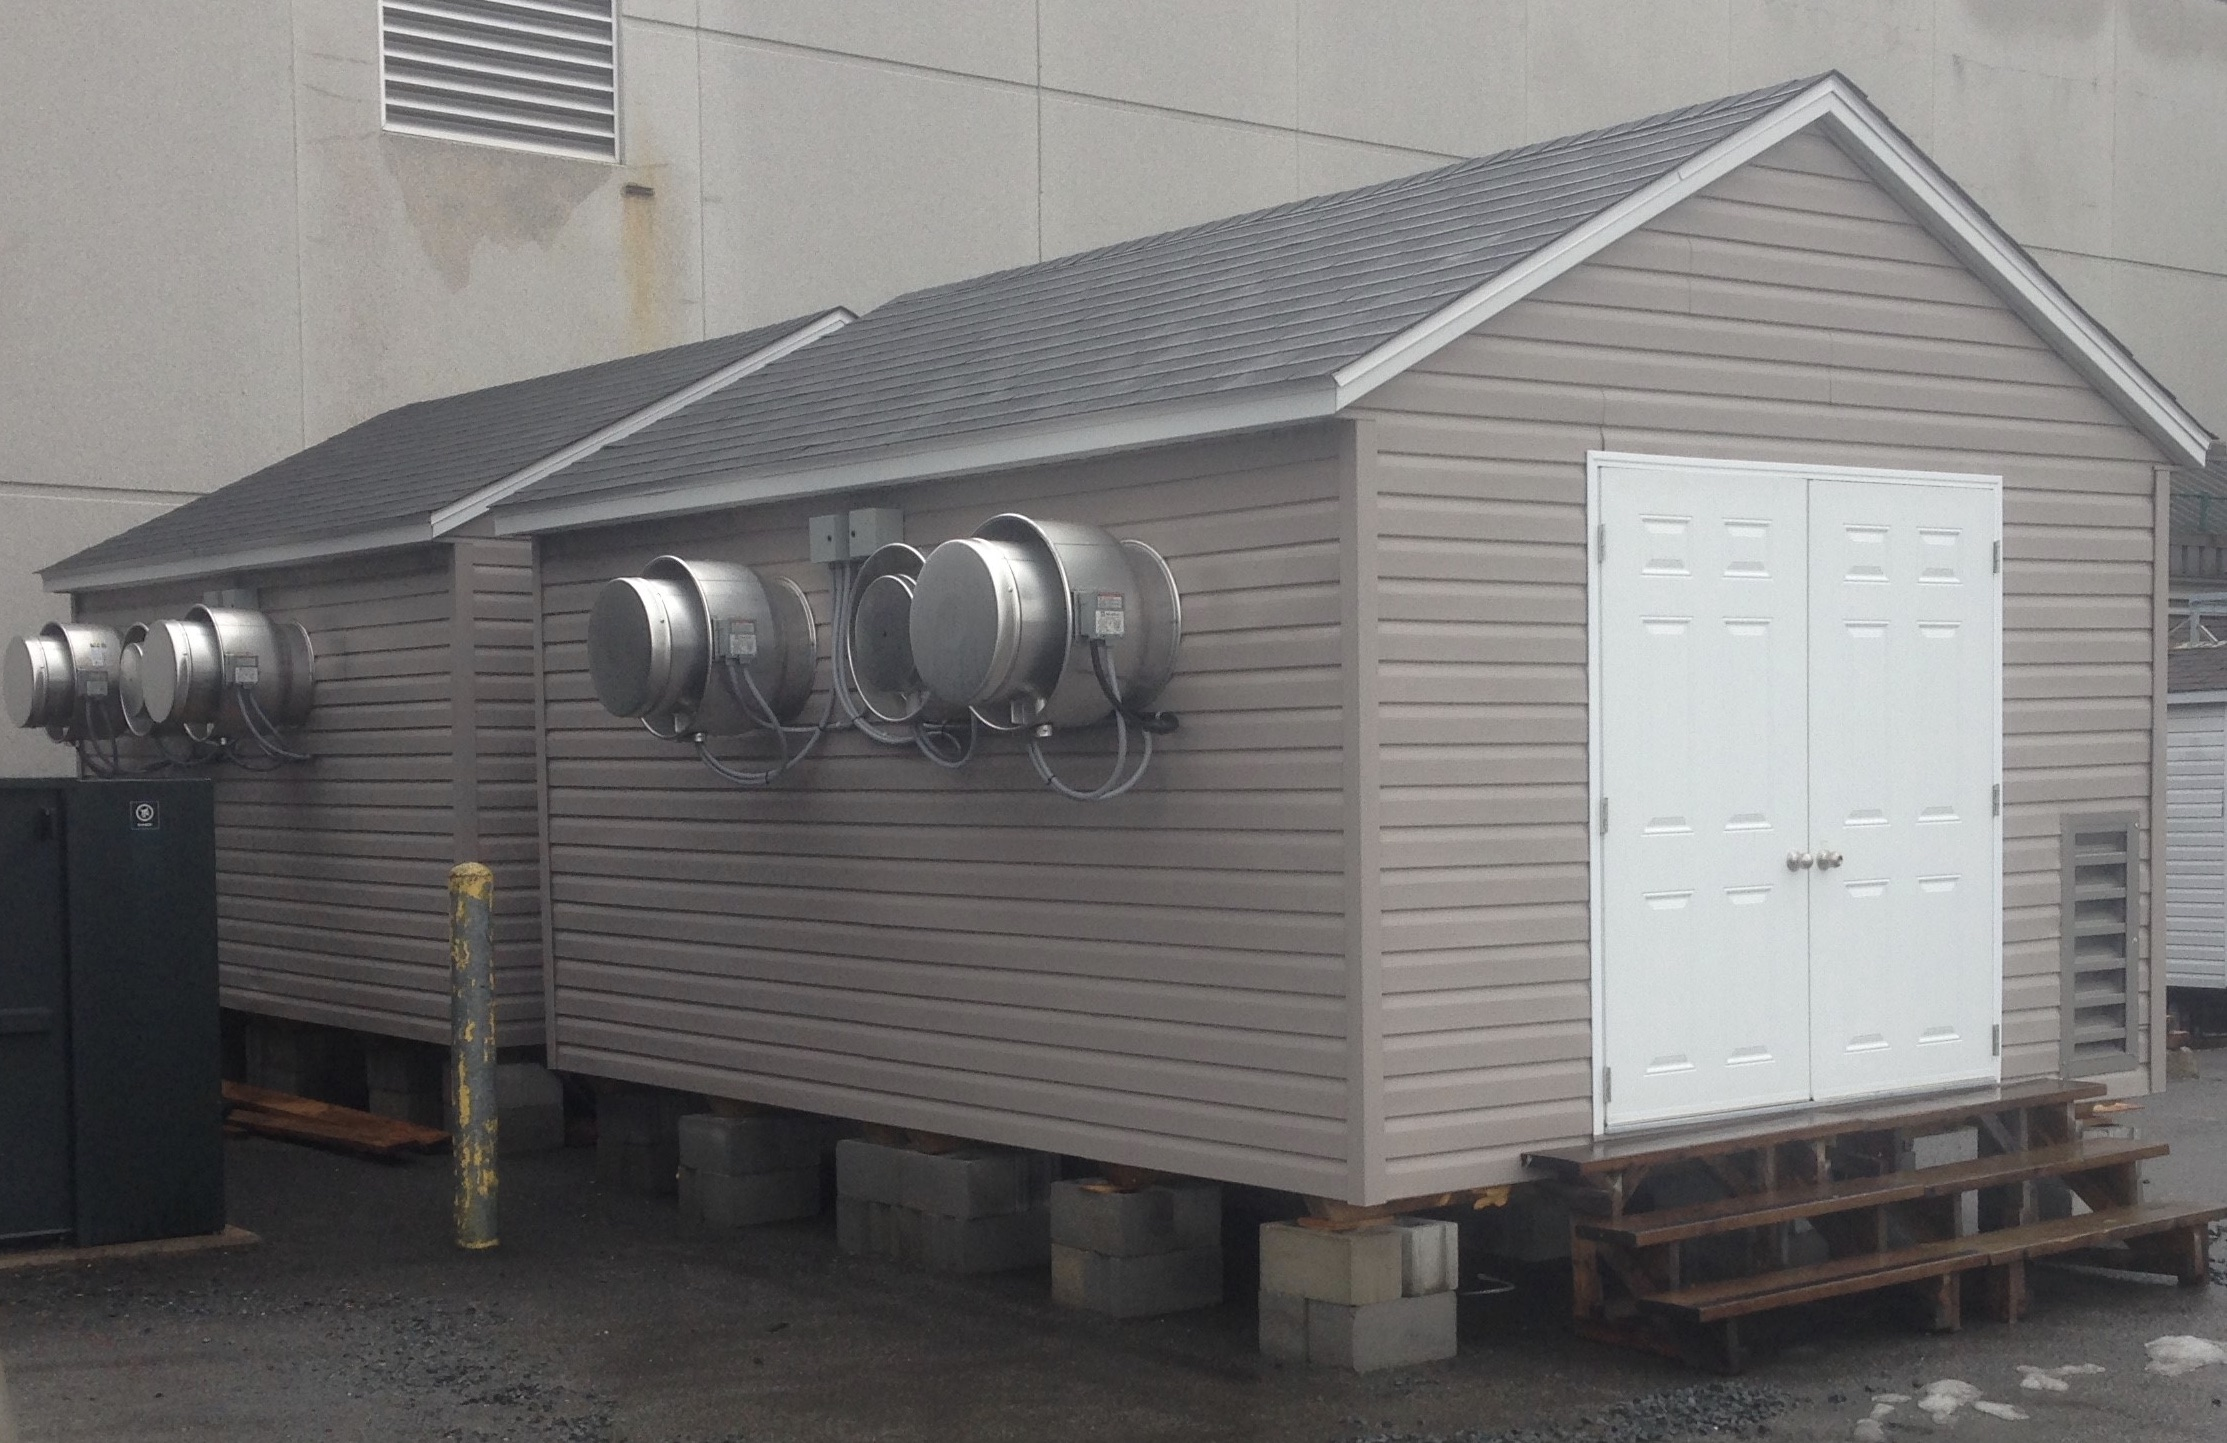
\includegraphics[width=2\colvsep]{pictures/sheds}};
\node[anchor=south west] at (p5cl cs:.25,0)
	{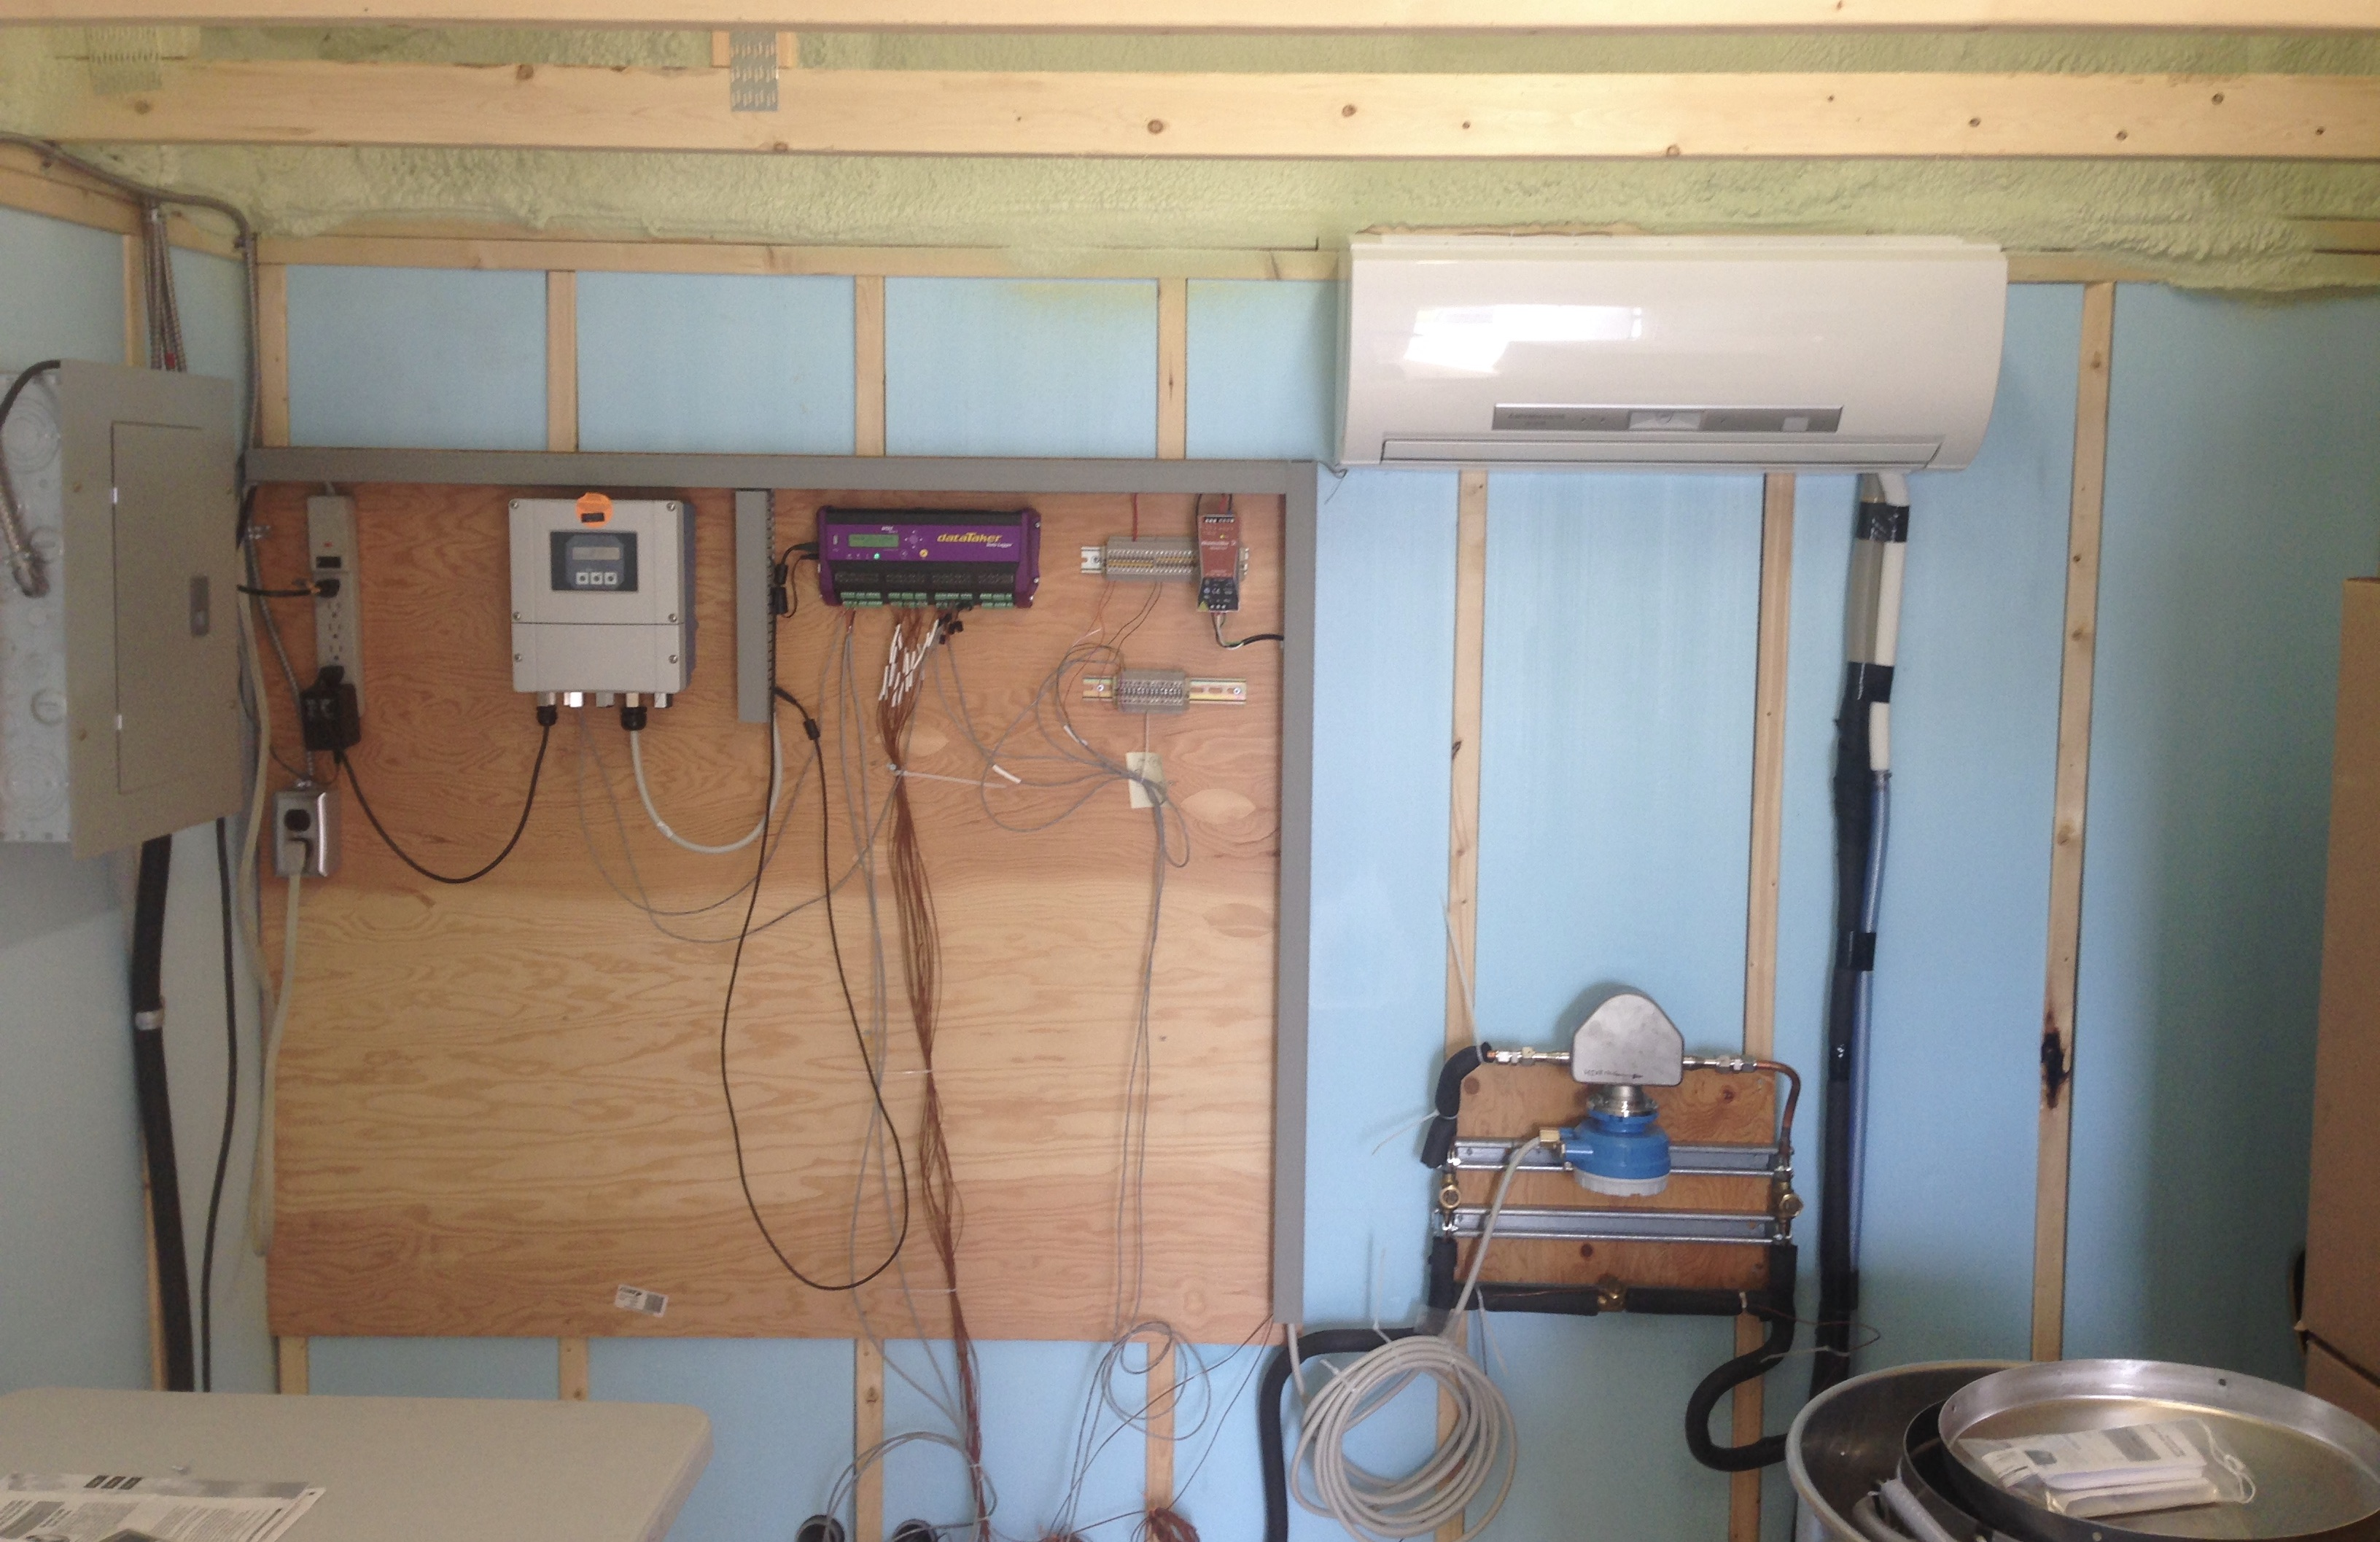
\includegraphics[width=2\colvsep]{pictures/indoor-unit}};
\node[anchor=south east] at (p5cr cs:3.75,0)
	{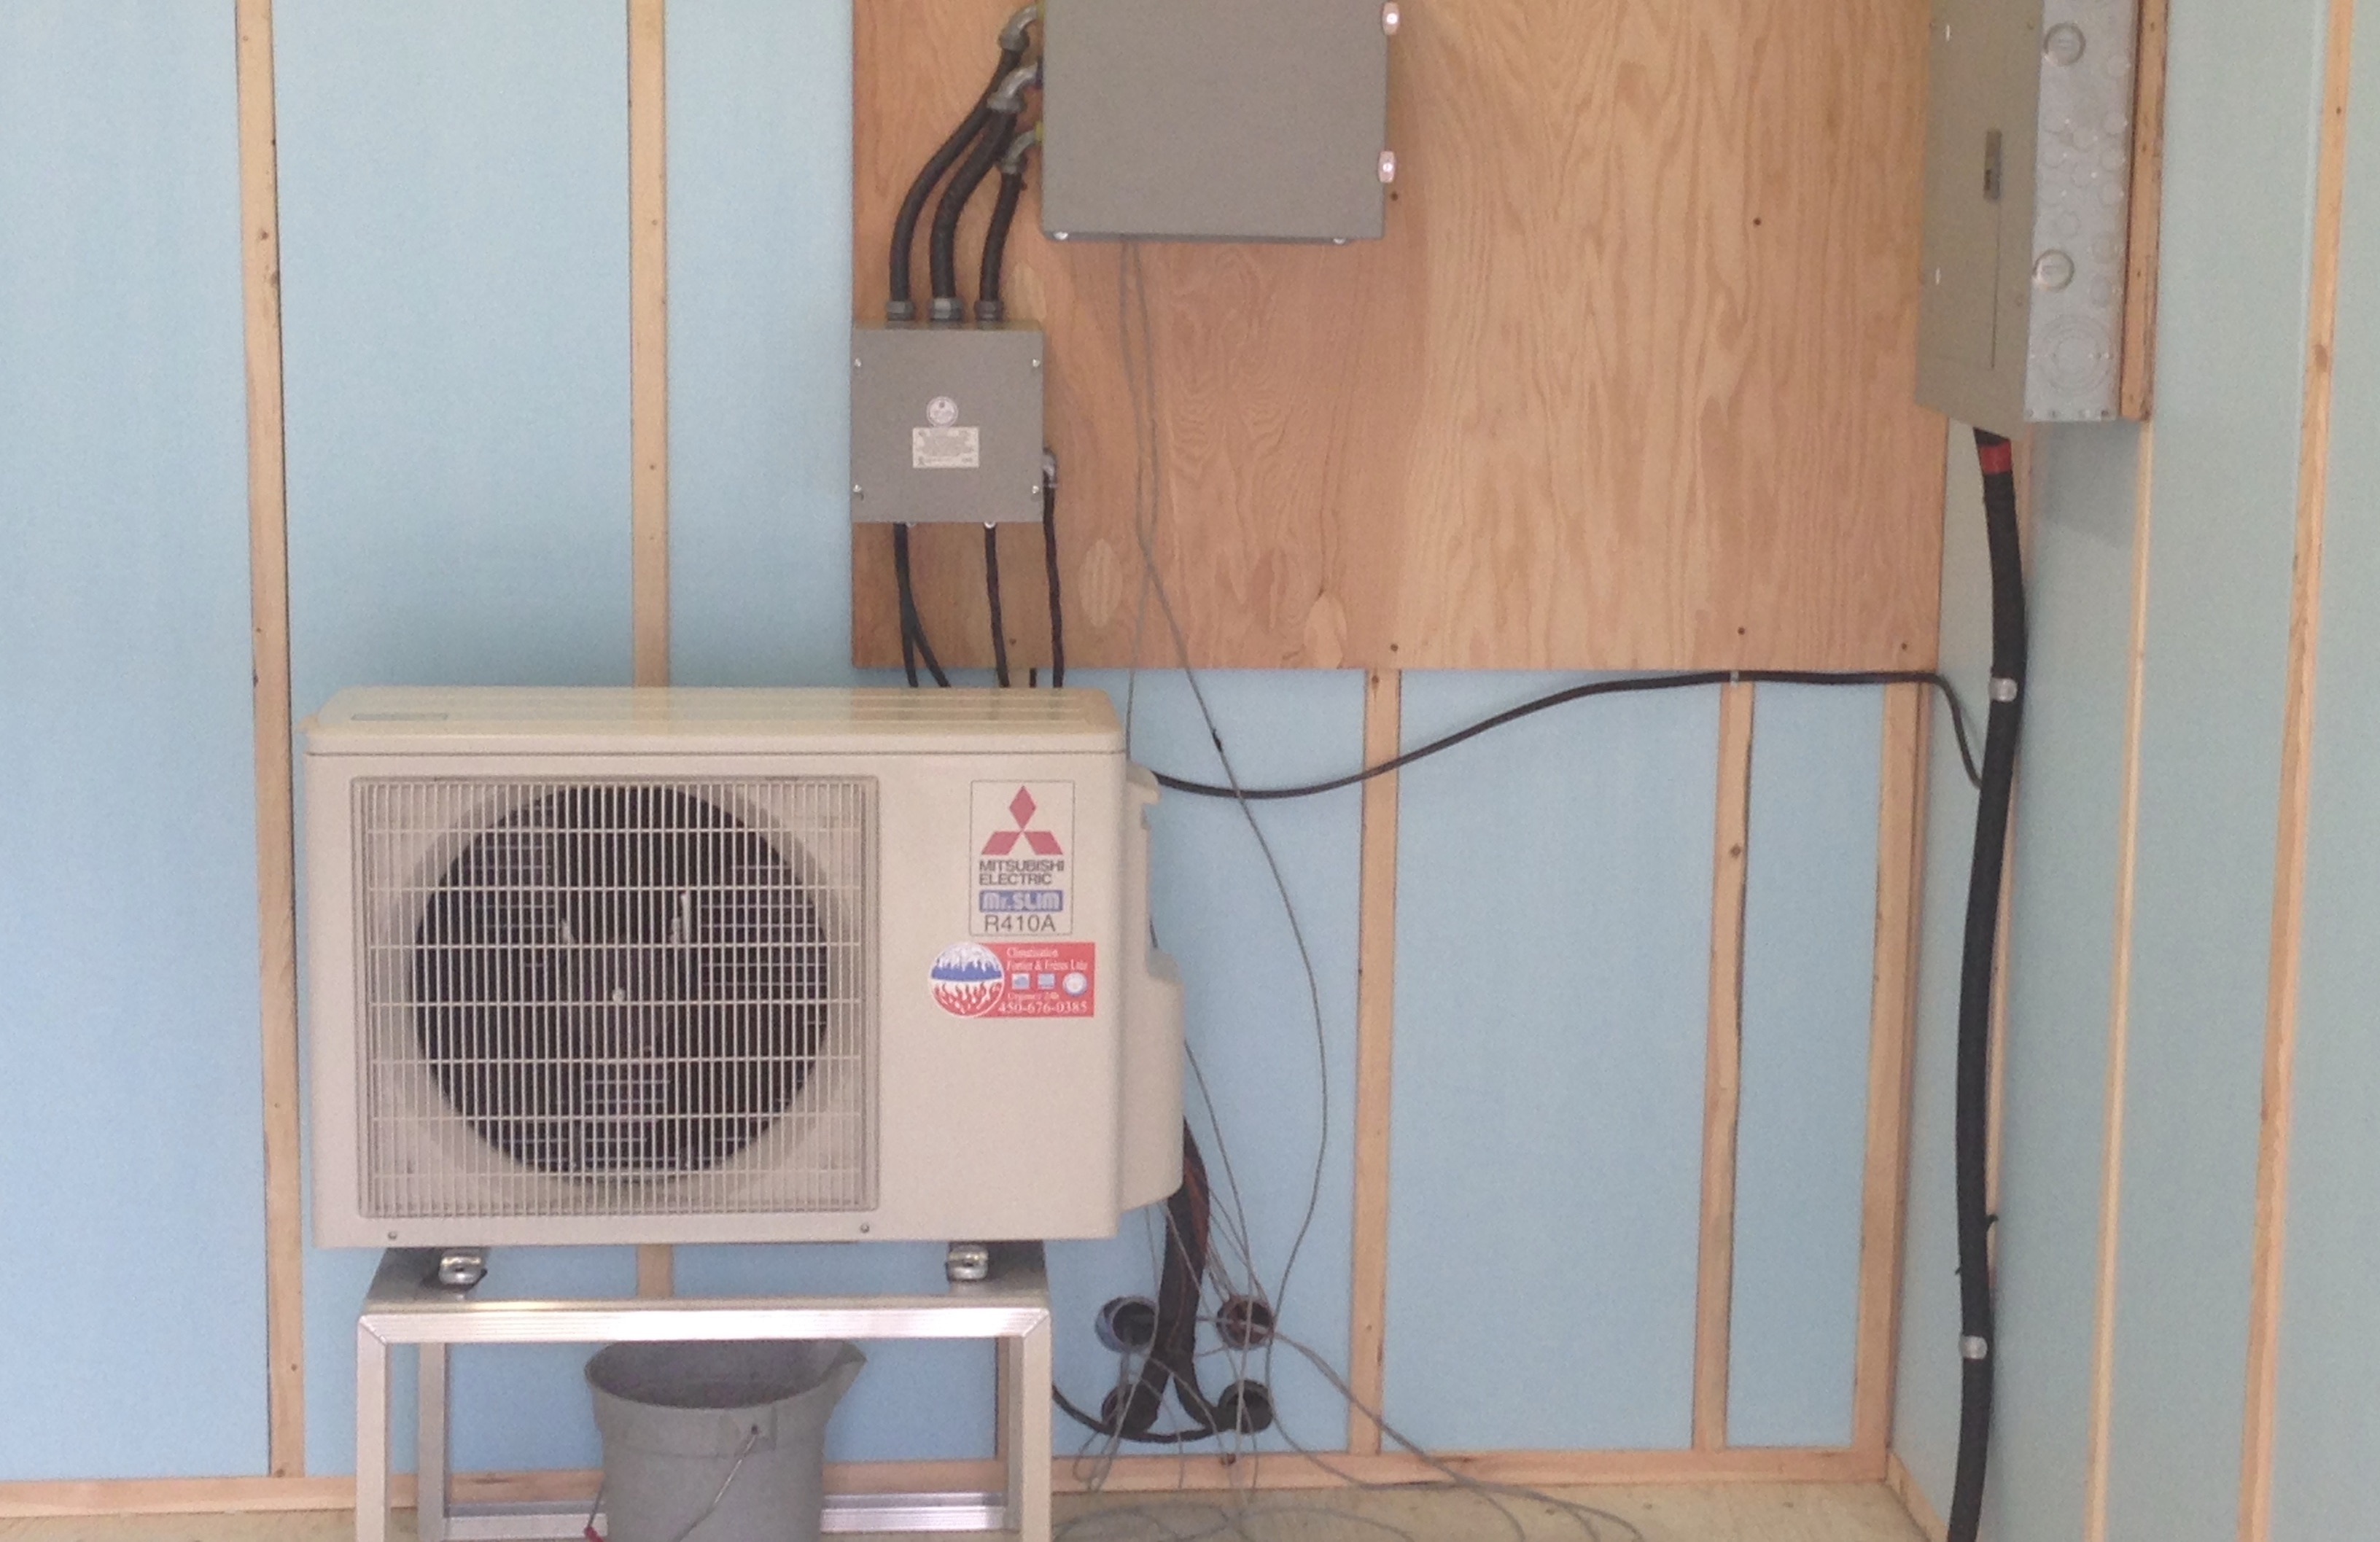
\includegraphics[width=2\colvsep]{pictures/outdoor-unit}};

\node[anchor=base east] at (t5cr cs:3.75,8){
	\begin{minipage}[b]{2\colvsep}
		Pour obtenir les performances dans les conditions désirées,
		\begin{listed}
		\setlength\itemsep{0pt}
			\item la charge
			\item la température extérieure
			\item le débit d'air
		\end{listed}
		sont imposés en contrôlant la quantité d'air entrant
	\end{minipage}};

\end{slide}



\begin{slide}[Le modèle parvient à prévoir les performances\\
			  \only<2>{et à reproduire les principaux comportements}]

\only<1>{
\begin{groupplot}[group style={group size=1 by 2,},
				  width=\bigcol+\colvsep,
				  xmin=0, xmax=3,
				  clip=false,
				  plot options,]
\nextgroupplot[
	height=3\baselineskip,
	axis x line=none,
	ymin=3.5, ymax=3.8,
	ytick={3.5, 3.8},
	yticklabels={3.5,\SI{3.8}{\kilo\watt}},
	at={(p5cr cs:1,10)},
	anchor=south west,
	]
\addplot[thick, gray] table[x=TIME, y=Qc-exp] {data/cooling-io.tsv};
\addplot[thick,  col] table[x=TIME, y=Qc-sim] {data/cooling-io.tsv};
\draw[latex-] (axis cs:1.7, 3.76) |- ++(3\quanta, 4\quanta)
	node[right, inner sep=3pt] {\footnotesize \SI{6.5}{\percent} error};
\draw[latex-] (axis cs:1.7, 3.5148) |- ++(0mm, -4\quanta);

\nextgroupplot[
	height=3\baselineskip,
	xtick={0, 3},
	xticklabels={0, \phantom{h\,}\SI{3}{\hour}},
	ymin=0.84, ymax=0.94,
	ytick={0.84, 0.94},
	yticklabels={840,\SI{940}{\watt}},
	at={(p5cr cs:1,3)},
	anchor=south west,
	]
\addplot[thick, gray] table[x=TIME, y=Pel-exp] {data/cooling-io.tsv};
\addplot[thick, col] table[x=TIME, y=Pel-sim] {data/cooling-io.tsv};
\draw[latex-] (axis cs:0.5833, 0.91648) |- ++(3\quanta, 4\quanta)
	node[right, inner sep=3pt] {\footnotesize \SI{8}{\percent} error};
\draw[latex-] (axis cs:0.5833, 0.84669) |- ++(0mm, -4\quanta);

\end{groupplot}

\node[anchor=mid west] at (p5cr cs:0,13) {\footnotesize\Qc};
\node[anchor=mid west] at (p5cr cs:0,6) {\footnotesize\Pel};
\node[gray, anchor=base west] at (t5cr cs:1.4,13.5)
	{\scriptsize measurements};
\node[col, anchor=base west] at (t5cr cs:1.4,9) {\scriptsize simulation};
}


\only<2>{
\begin{groupplot}[group style={group size=1 by 3,},
				  width=\bigcol+\colvsep,
				  xmin=0, xmax=4,
				  clip=false,
				  plot options,]
\nextgroupplot[
	height=3\baselineskip,
	axis x line=none,
	ymin=0, ymax=57,
	ytick={0, 57},
	yticklabels={0, \SI{57}{\hertz}},
	at={(p5cr cs:1,11)},
	anchor=south west,
	]
\addplot[thick, gray] table[x=TIME, y=f-exp] {data/cooling-sim.tsv};
\addplot[thick, col] table[x=TIME, y=f-sim] {data/cooling-sim.tsv};


\nextgroupplot[
	height=2\baselineskip,
	axis x line=none,
	ymin=14, ymax=24,
	ytick={14, 24},
	yticklabels={14, \SI{24}{\celsius}},
	at={(p5cr cs:1,7)},
	anchor=south west,
	]
\addplot[thick, gray] table[x=TIME, y=Ts-exp] {data/cooling-sim.tsv};
\addplot[thick, col] table[x=TIME, y=Ts-sim] {data/cooling-sim.tsv};
\draw[latex-] (axis cs:2.6, 17.373) |- ++(3\quanta, 4\quanta)
	node[right, inner sep=3pt] {\footnotesize\SI{3.7}{\celsius}};
\draw[latex-] (axis cs:2.6, 13.689) -- ++(0mm,-4\quanta);


\nextgroupplot[
	height=3\baselineskip,
	xtick={0, 4},
	xticklabels={0, \phantom{h\,}\SI{4}{\hour}},
	ymin=23, ymax=44,
	ytick={23, 44},
	yticklabels={23, \SI{44}{\celsius}},
	at={(p5cr cs:1,2)},
	anchor=south west,
	]
\addplot[thick] table[x=TIME, y=Toa] {data/cooling-sim.tsv}
	node[pos=0.7, fill=white, font=\footnotesize, inner sep=3pt] {\To};
\addplot[thick, gray] table[x=TIME, y=Tr-exp] {data/cooling-sim.tsv};
\addplot[thick, col] table[x=TIME, y=Tr-sim] {data/cooling-sim.tsv};

\end{groupplot}

\node[anchor=mid west] at (p5cr cs:0,14) {\footnotesize\fc};
\node[anchor=mid west] at (p5cr cs:0,9) {\footnotesize\Ts};
\node[anchor=mid west] at (p5cr cs:0,5) {\footnotesize\Tr};
}


\end{slide}

\begin{slide}[Les environnements intérieur et extérieur\\
			  sont chacun contrôlés dans un cabanon séparé]

\begin{scope}[shift={(p5cl cs:0,3)}, x=.25\bigcol, y=\baselineskip]

\node[anchor=base, gray] at (2, 10.25) {zone intérieure};
\fill[gray!20] (0,0) -| (4,6) -- (2,9)
			-- (0,6) |- (.2,5) |- (0,3.25) -- cycle;

% indoor unit
\node[minimum width=1cm, minimum height=3mm, rectangle, draw, thick,
	  rounded corners=.25\quantum] (IU) at (2.5,4.5) {};
\fill[gray!60!black] (IU.202) |- (IU.338 |- IU.west) |- cycle;
\path (.1,4.125) pic [rotate=90, thick] {fan=.4} node[dot, scale=1] {};

% points
\draw[latex-, col!50, thick] (IU.north) -- ++(0,1)
	node[dot, anchor=south, black, label={[black]above left:$r$}] (r) {};
\draw[-latex, col, thick] (IU.south) ++(0,.2) -- ++(0,-1)
	node[dot, anchor=north, black, label={[black]below left:$s$}] {};

% auxiliary heater
\draw[semithick] (0,.5) -- ++(.2,0)
	++(0,.16) rectangle ++(.6,-.33)++(0,.16)
	-| node[right, xshift=3pt] {\Lightning} ++(.2,-.5)
	foreach \x in {.35,.5,.65}{(\x,.66) -- (\x,.34)};

\end{scope}



\begin{scope}[shift={(p5cl cs:3,3)}, x=.25\bigcol, y=\baselineskip]

\node[anchor=base, gray] at (2, 10.25) {zone extérieure};
\fill[gray!20] (0,0) -| (4,3.25) -| (3.8,5) -| (4,6)
			-- (2,9) -- (0,6) -- cycle;
\path (3.9,4.125) pic [rotate=90, thick] {fan=.4} node[dot, scale=1] {};

% outdoor unit
\node[minimum width=1cm, minimum height=6mm, rectangle, draw, thick,
	  rounded corners=.25\quantum] (OU) at (1.5,2.3) {};
\node[circle, draw, minimum size=4\quanta] (grid) at ($(OU)-(.15,0)$) {};
\draw[ultra thin] foreach \angle in {-54, -36, ..., 54}{
	(grid.\angle) -- (grid.{180-\angle})
	(grid.{90+\angle}) -- (grid.{-90-\angle})};
\node[circle, fill=gray!60!black, scale=4]
	at ($(grid.east)!0.5!(OU.east)$) {};

% points
\coordinate (C1) at (2,0);
\node[dot, label={[black, yshift=3pt]above:$o$}] at (IU -| C1) {};

% auxiliary heater
\draw[semithick] (4,.5) -- ++(-.2,0)
	++(0,.16) rectangle ++(-.6,-.33)++(0,.16)
	-| node[left, xshift=-3pt] {\Lightning} ++(-.2,-.5)
	foreach \x in {.35,.5,.65}{(4-\x,.66) -- (4-\x,.34)};

\end{scope}


% refrigerant lines
\only<1>{
\draw[col, midarrow=0.5-latex, semithick] (OU.west)++(0,.05)
	-| ($(IU.east)+(.55,.05)$) -- ($(IU.east)+(0,.05)$);
\draw[gray, midarrow=0.65-latex, semithick] (IU.east)++(0,-.05)
	-- ++(.45,0) |- ($(OU.west)-(0,.05)$);
}
\only<2>{
\draw[gray, midarrow=0.65-latex, semithick] (IU.east)++(0,.05) -- ++(.55,0)
	|- ($(OU.west)+(0,.05)$);
\draw[col, midarrow=0.5-latex, semithick] (OU.west)++(0,-.05)
	-| ($(IU.east)+(.45,-.05)$) -- ($(IU.east)-(0,.05)$);
}

% heat flux
\only<1>{
\node[becomes, rotate=90, anchor=south,
	  label={[left, label distance=\quantum]:\Qh}]
	at ($(IU.west)-(2\quanta,0)$) {};
\node[becomes, rotate=90, anchor=north,
	  label={[right, xshift=3.5\quanta]:$\skew{5}\dot Q_\text{abs}$}]
	at ($(OU.east)+(2\quanta,0)$) {};
}
\only<2>{
\node[becomes, rotate=-90, anchor=north,
	  label={[left, xshift=-3.5\quanta]:\Qc}]
	at ($(IU.west)-(2\quanta,0)$) {};
\node[becomes, rotate=-90, anchor=south,
	  label={[right, xshift=\quantum]:$\skew{5}\dot Q_\text{rej}$}]
	at ($(OU.east)+(2\quanta,0)$) {};
}

\end{slide}




\begin{slide}[Le débit d'air de l'unité intérieure\\
			  est mesuré avec un \emph{duct blaster}]


\begin{scope}[shift={(p5cl cs:0.3,6)}]

% air flux
\draw[line width=1mm, -{Triangle[scale=0.7]}, col!50] (.2,3.4)
	node[above, yshift=1mm, black] {$r$} to[out=270, in=110] (.35,2.4);
\draw[line width=1mm, -{Triangle[scale=0.7]}, col] (.4,2.25)
	to[out=320, in=180] (1.4,1.95) node[right, black, xshift=1mm] {$s$};

% indoor unit
\filldraw[gray!50, very thick] (0,3) rectangle (-.2,2);
\draw[dotted] (0,3) -- (0.5,3);
\draw[very thick, line cap=rect] (.5,3) -- (1,3) node (IU) {}
									 to[out=270, in=60] (.9,2.3)
								 (0,3) |- (0.5,2) -- ++(340:.2)
								 (.75,2.15) -- ++(340:.2);

% plenum
\draw[semithick] (1,2.8) -- (2,2.8) -- (3,2.5)
	  (.25,2) |- (2,1) -- (3,1.3);

% join
\filldraw[semithick] (3,2.5) rectangle (3.2,1.3);

% duct
\draw[semithick, gray] (3.2,2.5) arc (90:20:2.2) -- ++(290:1.5)
	arc(200:270:1) node (N0) {} -- ++(1.2,0) node (N1) {};
\draw[semithick, gray] (3.2,1.3) arc (90:20:1) -- coordinate (C1)
	++(290:1.5) arc (200:270:2.2) -- ++(1.2,0) node (N2) {};
\draw[gray] foreach \theta in {20, 30, ..., 90}{
				(3.2,.3)++(\theta:1) -- ++(\theta:1.2)}
            foreach \x in {0.3, 0.6, ..., 1.5}{
            		(3.2,.3)++(20:1)++(290:\x) -- ++(20:1.2)}
            foreach \theta in {200, 210, ..., 270}{
            		(N0)++(0,1)++(\theta:1)    -- ++(\theta:1.2)}
            foreach \x in {0.3, 0.6, 0.9}{
            		(N0)++(\x,0) -- ++(0,-1.2)};

% join
\filldraw[thick] (N1)++(.2,0) rectangle (N2);

% fan casing
\draw[thick] (N1)++(.2,0) arc (270:360:.1) |- node (D1) {} ++(.7,.2)
		-- ++(0,-.3) node (P1) {}
			 (N2)++(.2,0) arc (90:0:.1)    |- ++(.7,-.2) node (D2) {}
		-- ++(0,.3) node (P2) {};

\draw foreach \y in {-.45,-.3,...,.45}{
	($(P1)!0.5!(P2)-(.05,\y)$) -- ++(.1,0) };

% fan
\path ($(D1)!0.5!(D2)$) pic [rotate=90, thick] {fan2=2} node[dot] (F) {};

% outlet air flux
\draw[line width=1mm, -{Triangle[scale=0.7]}, col] ($(P1)!0.5!(P2)+(.2,0)$) -- ++(.7,0);

% labels
\draw[gray, semithick] (IU)++(45:3pt) -- ++(45:.7) -- ++(.7,0)
	node[anchor=mid west, inner sep=3pt] {unité intérieure};

\draw[gray, semithick] (D1.north -| F)++(0,3pt) -- ++(0,1)
	node[above, inner sep=3pt] {duct blaster};

\draw[gray, semithick] (C1)++(200:3pt) -- ++(200:.7) -- ++(-.7,0)
	node[anchor=mid east, inner sep=3pt] {conduit flexible};

\end{scope}

\end{slide}





\setlength{\templen}{7\baselineskip}

\begin{slide}[Les capacités totales sont plus facilement calculées\\
			  avec les propriétés du réfrigérant]


\begin{scope}[shift={(p5cl cs:0,4)}, visible on=<{1,4-5}>]

% four-way valve 
\coordinate [circle, draw, thick, minimum size=7mm]
	(4wValve) at (\templen, 0.5\templen) {};

% compressor
\coordinate [compressor, draw, thick, minimum size=7mm,
			 right=\bigcol-\templen of 4wValve.center, anchor=center]
	(comp);

% indoor unit HX
\draw[thick, HX] (0.5\templen-5mm,\templen) node (iuOut) {} --
	node [yshift=2\baselineskip, gray] {\scriptsize unité intérieure}
	++(1,0) node (iuIn) {};

% expansion valve
\coordinate [expValve] (v) at (0,0.5\templen) {};

% outdoor unit HX
\draw [HX, thick] (0.5\templen-5mm,0) node(ouIn){} --
	node [yshift=-2\baselineskip, gray] {\scriptsize unité extérieure}
	++(1,0) node (ouOut) {};

% refrigerant lines, heating
\begin{scope}[visible on=<{1,4}>]

\draw[thick, midarrow=.75-latex, col!50]
	(ouOut.center) -| coordinate (6h) (4wValve.225);
\coordinate (C0) at ($(4wValve.225)!0.5!(ouOut)$);
\draw[thick, col!50, line cap=rect]
	(4wValve.225)++(0,-.1) -- (4wValve.225)
	arc (135:45:3.5mm) -- (C0 -| 4wValve.315) coordinate (C1);
\draw[thick, midarrow=.4-latex, col!50]
	(C1) -| coordinate (1) (comp.south);
\coordinate (C2) at ($(4wValve.45)!0.5!(iuIn)$);
\draw[thick, midarrow=.5-latex, col]
	(comp.north) |- coordinate (2) (4wValve.135 |- C2) -- (4wValve.135);
\draw[thick, col] (4wValve.135)++(0,.1) -- ++(0,-.1) arc (225:315:3.5mm)
	coordinate (C3) -- ($(2 -| C3)-(0,.05)$) ++(0,.1) coordinate (C4);
\draw[thick, midarrow=.75-latex, col]
	(C4) |- coordinate (3) (iuIn.center);
\draw[thick, midarrow=.8-latex, gray]
	(iuOut.center) -| coordinate (4) (v.north);
\draw[thick, midarrow=.85-latex, gray!50]
	(v.south) |- coordinate (5h) (ouIn.center);

\end{scope}

% refrigerant lines, cooling
\begin{scope}[visible on=<5>]

\coordinate (C0) at ($(4wValve.225)!0.5!(ouOut)$);
\coordinate (C2) at ($(4wValve.45)!0.5!(iuIn)$);
\draw[thick, midarrow=.5-latex, col]
	(comp.north) |- coordinate (2) (4wValve.135 |- C2) -- (4wValve.135);
\draw[thick, col, midarrow=.53-latex] (4wValve.135)++(0,.1) -- ++(0,-.1)
	arc (45:-45:3.5mm) |- coordinate (6) (ouOut.center);
\draw[thick, midarrow=.8-latex, gray]
	(ouIn.center) -| coordinate (5) (v.south);
\draw[thick, midarrow=.85-latex, gray!50]
	(v.north) |- coordinate (4c) (iuOut.center);
\draw[thick, midarrow=.3-latex, col!50] (iuIn.center) -| coordinate (3c)
	($(C2 -| 4wValve.45)+(0,.05)$) ++(0,-.1) -- (4wValve.45);
\draw[thick, col!50, line cap=rect] (4wValve.45)++(0,.1) -- ++(0,-.1)
	arc (135:225:3.5mm) -- (C0 -| 4wValve.315) coordinate (C1);
\draw[thick, col!50, midarrow=.4-latex] (C1) -| coordinate (1) (comp.south);

\end{scope}

% re-draw valve to avoid overlap
\node[expValve, thick] at (v) {};

\tikzset{inner sep=3pt, font=\scriptsize}
% refrigerant states
\foreach \sensor/\lab/\pos in {1/1/below right, 2/2/above right,
							   3/3/above right, 4/4/above left,
							   5h/5/below left, 6h/6/below right}{
	\node[dot, label=\pos:\lab] at (\sensor) {};}

\end{scope}


\node[anchor=base west, visible on=<{2-3,6}>,
	  background text=gray, text on=<{3,6}>] at (t5cl cs:0,9)
	{$ \Pcp = \mr(h_2 - h_1) $};
\node[anchor=base west, visible on=<{3,6}>,
	  background text=gray, text on=<6>] at (t5cl cs:0,7)
	{$ \Qh = \mr(h_3 - h_4) + \Pfi $};
\node[anchor=base west, visible on=<6>] at (t5cl cs:0,5)
	{$ \Qc = \mr(h_3 - h_4) - \Pfi $};


\begin{scope}[shift={(p5cl cs:3,5)}, x=\bigcol/5,
			  y=4\baselineskip/1.7183, xshift=.1\bigcol]

\tikzset{inner sep=3pt, font=\scriptsize}

\coordinate (LVEbottom) at (2.4,-\baselineskip);
\fill[gray!20] (-.5,-\baselineskip) to [out=65, in=220] (1,2.65)
	to [out=40,in=180] (1.6,2.8) coordinate (SC)
	to [out=0, in=80] coordinate[pos=0.3] (LVE) (LVEbottom);
\only<1>{
	\node[gray, align=left, font=\scriptsize, anchor=base east]
		(LVElab) at (t5cr cs:4,12) {Équilibre\\liquide-vapeur};
	\draw[gray] (LVElab.base -| LVElab.230)++(0,-3pt) -- ++(0,-.4)
		coordinate (C1) -- ($(C1)!0.8!(LVE)$);}

\draw[midarrow=0.55-latex, hl=draw on <6>]
	(0,0) coordinate[dot, hl=fill on <6>] (evi) --
	(2.6,0) coordinate[dot, hl=fill on <6>] (evo);
\draw (evo) -- (3,0) coordinate (cpi);
\draw[midarrow=0.55-latex, hl=draw on <2>]
	(cpi) node[dot, hl=fill on <2>] {} --
	plot[domain=3:4.5] (\x, {exp(\x/1.5-2) - 1})
	coordinate[dot, hl=fill on <2>] (cpo);
\draw (cpo) -- ++(-.5,0) coordinate[dot, hl=fill on <3>] (cdi);
\draw[midarrow=0.5-latex, hl=draw on <3>] (cdi) -- (cpo -| evi)
	coordinate[dot, hl=fill on <3>] (cdo) {};
\draw[midarrow=0.55-latex] (cdo) -- (evi);

\node [below right, background text=col, text on=<2>] at (cpi) {1};
\node [above right, background text=col, text on=<2>] at (cpo) {2};
\node [above, background text=col, text on=<3>] at (cdi)
	{\temporal<4>{3}{3}{6}};
\node [above left, background text=col, text on=<3>] at (cdo)
	{\temporal<4>{4}{4}{5}};
\node [below left, background text=col, text on=<6>] at (evi)
	{\temporal<4>{5}{5}{4}};
\node[below, background text=col, text on=<6>] at (evo)
	{\temporal<4>{6}{6}{3}};


% axes
\draw[semithick, hlb=draw on <{3,6}>]
	(0,-8\quanta) node[below, hlb=text on <{3,6}>] {$ h_4 $}
	++(-.3pt,0) -- (2.6,-8\quanta) -- ++(.3pt,0);
\draw[semithick, hlb=draw on <3>] (2.6,-8\quanta)
	node[below, hlb=text on <6>] {$ h_{\temporal<4>{6}{6}{3}} $}
	++(.3pt,0) -- ($(3,-8\quanta)-(.3pt,0)$);
\draw[semithick, hlb=draw on <{2,3}>]
	(3,-8\quanta) node[below, hlb=text on <2>] {$ h_1 $}
	++(-.3pt,0) -- (4,-8\quanta) -- ++(.3pt,0);
\draw[semithick, hlb=draw on <2>] (4,-8\quanta)
	node[below, hlb=text on <3>] {$ h_{\temporal<4>{3}{3}{6}} $}
	++(.3pt,0) -- (4.5,-8\quanta) node[below, hlb=text on <2>] {$ h_2 $}
	-- ++(.3pt,0);
\draw[semithick, hlb=draw on <{3,6}>]
	(0,-8\quanta)++(0,.3pt) -- (0,-7\quanta);
\draw[semithick, hlb=draw on <6>]
	(2.6,-8\quanta)++(0,.3pt) -- (2.6,-7\quanta);
\draw[semithick, hlb=draw on <2>]
	(3,-8\quanta)++(0,.3pt) -- (3,-7\quanta);
\draw[semithick, hlb=draw on <3>]
	(4,-8\quanta)++(0,.3pt) -- (4,-7\quanta);
\draw[semithick, hlb=draw on <2>]
	(4.5,-8\quanta)++(0,.3pt) -- (4.5,-7\quanta);

\draw[gray, semithick]
	(-7\quanta,0) -| node[left] {$ p_{\temporal<4>{5}{5}{4}} = p_1 $}
	(-8\quanta,1.7183) node[left] {$ p_{\temporal<4>{4}{4}{5}} = p_2 $}
	-- +(\quantum,0);

\end{scope}

\end{slide}





\end{document}
